% ===================================================================== %
%  Apresentação de TCC — Ciência da Computação / IC-UFAL
%  José Félix de Oliveira Neto
%
%  Classe: UFAL-beamer-moderno.cls  (opções: 43, helvet)
%  Compilar: latexmk -pdf main   (ou pdflatex x2 — a barra de progresso
%            e o total de páginas precisam de duas passadas)
% ===================================================================== %
\documentclass{UFAL-beamer-moderno}

\usepackage{booktabs}
\graphicspath{{img/}{../Monografia/Cap04/img/}{../Monografia/Cap05/img/}}

% --------------------------------------------------- %
%                  Informações                         %
% --------------------------------------------------- %
\doctype{Trabalho de Conclusão de Curso}
\title[NAS robusta para TinyML]{Busca Arquitetural Neural para TinyML por
validação de robustez}
\subtitle{Uma adaptação do Once-for-All}
\author[José Félix]{José Félix de Oliveira Neto}
\supervisor{Prof. Dr. Erick de Andrade Barboza}
\institute[IC/UFAL]{Instituto de Computação --- Universidade Federal de Alagoas}
\date[Nov/2026]{Maceió, novembro de 2026}
\ufallogo{IC.jpg}

\begin{document}

\titlepage

\begin{frame}{Roteiro}
  \tableofcontents[hideallsubsections]
\end{frame}

% ===================================================================== %
\section{Introdução}
% ===================================================================== %

\begin{frame}{Motivação}{Modelos compactos precisam funcionar fora do laboratório}
  \begin{columns}[T]
    \begin{column}{0.55\textwidth}
      \begin{itemize}
        \setlength{\itemsep}{8pt}
        \item Dispositivos \emph{TinyML} têm poucos KB de memória
        \item NAS (ex.: Once-for-All) encontra subredes eficientes\ldots
        \item \ldots mas otimiza só a acurácia em imagens \textbf{limpas}
          \begin{itemize}
            \item ruído, desfoque, mudanças de iluminação
          \end{itemize}
      \end{itemize}
      \vspace{6pt}
      \notebox{\textbf{Hipótese:} incluir robustez na \textit{fitness} da busca
      evolutiva estabiliza a seleção de subredes.}
    \end{column}
    \begin{column}{0.40\textwidth}
      \centering
      \bignumber{+X,X p.p.}{MCA da melhor subrede\\(valor ilustrativo)}
      \vspace{10pt}
      \alertbox{\small Robustez não é avaliada na busca padrão.}
    \end{column}
  \end{columns}
\end{frame}

\begin{frame}{Objetivos}
  \begin{block}{Objetivo geral}
    Avaliar e melhorar a robustez de subredes extraídas pela técnica evolutiva do
    Once-for-All sob corrupções naturais de imagem.
  \end{block}
  \vspace{6pt}
  \begin{enumerate}
    \setlength{\itemsep}{6pt}
    \item Construir o conjunto VWW-C (Visual Wake Words corrompido)
    \item Treinar um \textit{Robustness Predictor} para estimar a MCA
    \item Incorporar robustez à \textit{fitness} e comparar com o baseline
  \end{enumerate}
\end{frame}

% ===================================================================== %
\section{Fundamentação Teórica}
% ===================================================================== %

\begin{frame}{Blocos e destaques}
  \begin{columns}[T]
    \begin{column}{0.48\textwidth}
      \begin{block}{Bloco padrão}
        Conceito ou definição.
      \end{block}
      \begin{exampleblock}{Exemplo}
        Resultado positivo.
      \end{exampleblock}
      \begin{alertblock}{Atenção}
        Limitação ou ressalva.
      \end{alertblock}
    \end{column}
    \begin{column}{0.48\textwidth}
      \notebox{\texttt{\textbackslash notebox}: nota neutra, sem título.}
      \goodbox{\texttt{\textbackslash goodbox}: conclusão positiva.}
      \alertbox{\texttt{\textbackslash alertbox}: alerta.}
      \[ \text{MCA} = \frac{1}{|C|}\sum_{c\in C}\frac{1}{5}\sum_{s=1}^{5} \text{Acc}_{c,s} \]
    \end{column}
  \end{columns}
\end{frame}

% ===================================================================== %
\section{Metodologia}
% ===================================================================== %

\begin{frame}{Ciclo evolutivo}
  \centering
  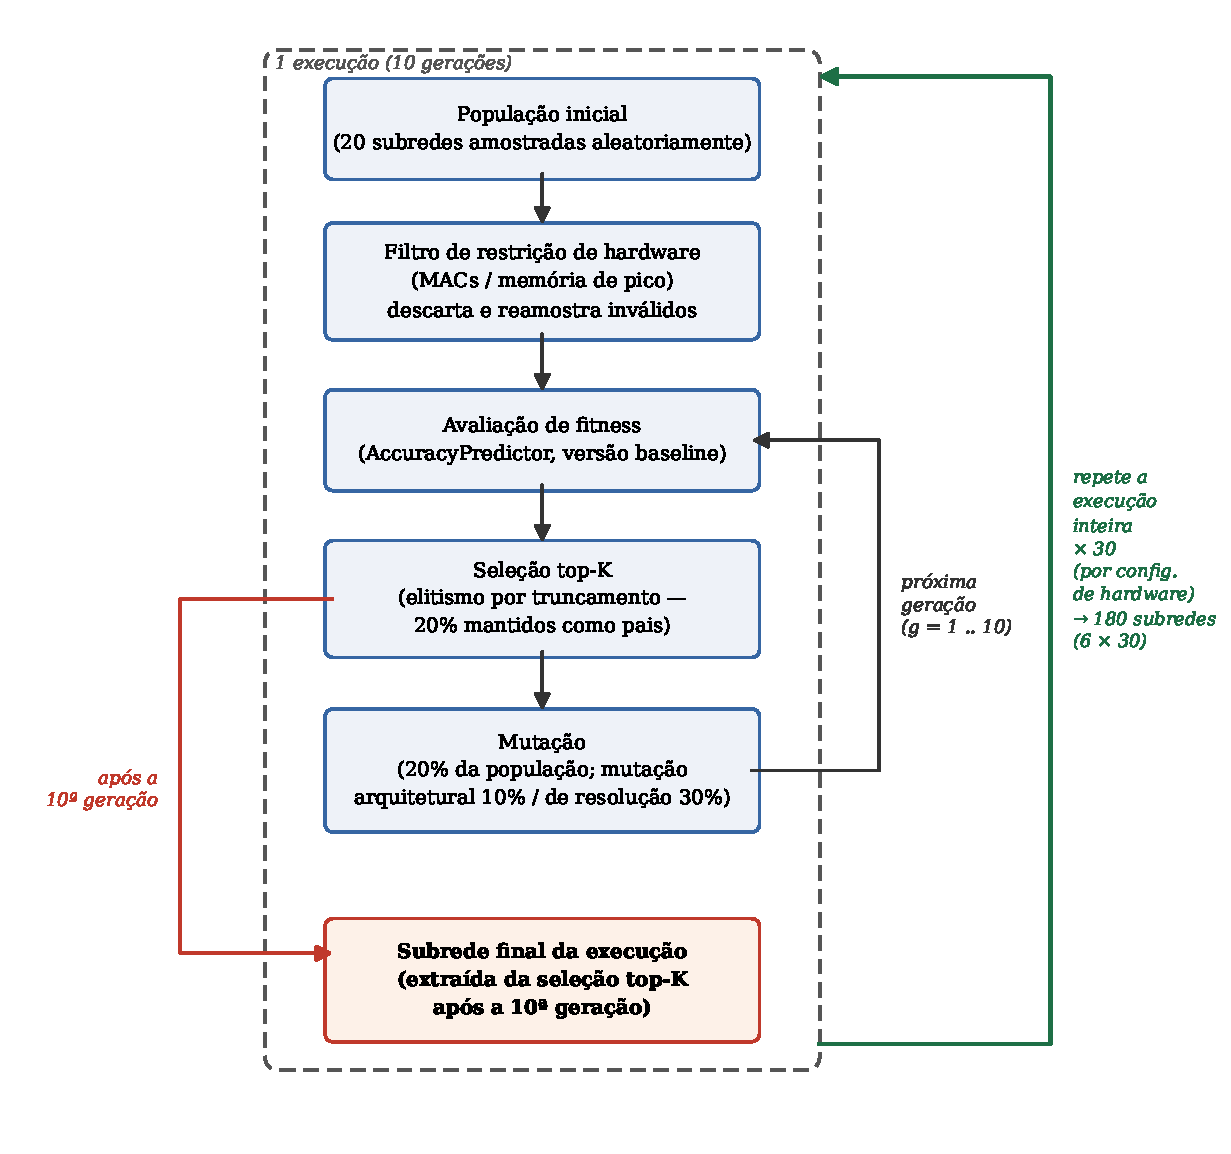
\includegraphics[height=0.62\textheight]{evolutionary_cycle_flowchart.pdf}\\[2pt]
  \src{Elaborado pelo autor}
\end{frame}

% ===================================================================== %
\section{Resultados}
% ===================================================================== %

\begin{frame}{Tabela de exemplo}
  \centering
  \begin{tabular}{lccc}
    \toprule
    \textbf{Fitness} & \textbf{Acc. limpa} & \textbf{MCA} & \textbf{Latência} \\
    \midrule
    Baseline     & 00,0\% & 00,0\% & 0,0 ms \\
    Robust       & 00,0\% & \textcolor{ufalBlue}{\textbf{00,0\%}} & 0,0 ms \\
    Weighted     & 00,0\% & 00,0\% & 0,0 ms \\
    \bottomrule
  \end{tabular}\\[6pt]
  \src{valores fictícios}
\end{frame}

% ===================================================================== %
\section{Conclusão}
% ===================================================================== %

\begin{frame}{Considerações finais}
  \begin{itemize}
    \setlength{\itemsep}{8pt}
    \item Contribuição 1
    \item Contribuição 2
    \item Trabalhos futuros
  \end{itemize}
\end{frame}

\end{document}
